\documentclass{scrreprt}
\usepackage[utf8]{inputenc}

\usepackage{natbib}
\usepackage{graphicx}
\usepackage{tikz}
\usepackage{pgfplots}
\pgfplotsset{compat=1.12}
\usepackage{textcomp}

\usepackage{amsmath} % Math
\usepackage{hyperref} % Hyperlinks
\usepackage[noabbrev]{cleveref} % Clickable hyperlinks
\usepackage[parfill]{parskip} % Remove intent on paragraph
\usepackage{caption} % add captions
\usepackage{url} % URLs
\usepackage{pdfpages} %add pdf as pages

\usepackage{glossaries} % for abbreviation list
%\usepackage[doublespacing]{setspace}
%\usepackage[nopostdot,style=super,nonumberlist,toc]{glossaries}

\renewcommand{\baselinestretch}{1.5}

% Edit the meta.tex file to change title and author names

\usepackage{tocbibind} % fix for wrong hyperlink for toc, tof and tot

\newcommand{\mytitle}{\textbf{A Control System for Autonomous Vehicles}\par
Forward and Inverse Kinematics}
\newcommand{\myauthor}{Stefan Bui}
\newcommand{\mysupervisor}{Sven Fjeldass}

\title{\mytitle}
\author{\myauthor}
\date{\today}

% Source of figures
\newcommand*{\captionsource}[1]{
    \fontsize{7}{6}\selectfont{
        \hspace{\linewidth}
        \textbf{Source:} #1
    }
}

% Fix stuff with glossary and koma-script
\AtBeginDocument{%
  \setlength{\glsdescwidth}{0.8\columnwidth}%
  \setlength{\glspagelistwidth}{.1\columnwidth}%
}

\newglossarystyle{custom_super}
{
    \setglossarystyle{long3colheader}%
    \renewcommand*{\glossaryheader}{}%  
    \renewcommand{\glossentry}[2]{%
        \textbf{\glsentryitem{##1}\glstarget{##1}{\glossentryname{##1}}}
        & \glossentrydesc{##1}
        & ##2
        \tabularnewline}%
}

\makeglossaries

\newglossaryentry{AUV}
{
        name=AUV,
        description={Autonomous underwater vehicle}
}

\newglossaryentry{End-effector}
{
        name=End-effector,
        description={The device at the end of a robotic arm}
}


\newglossaryentry{Basis}
{
        name=Basis,
        description={A set of unit vectors pointing in a space in a Cartesian coordinate system}
}

\newglossaryentry{TGroup}
{
        name=TGroup,
        description={A class in GeoMod that contains geometric data with designated coordinate frame eometric data with designated coordinate frame}
}

\newglossaryentry{Workspace}
{
        name=Workspace,
        description={The volume of space a robot's end-effector can reach, limited by its joints and presence of obstacles}
}


%----- DOCUMENT -----
\begin{document}

% The title page
\begin{titlepage}

\begin{center}
    
    ~\\[2.0cm]
    
    \Large \textbf{Semester project}\\[2.5cm]
     
    % Set the title of the Document between two horizontal lines
    \hrule
    {\LARGE \mytitle}	% print the title of the document
    \vspace{0.5cm}
    \hrule
    
    \vspace{1.0cm}
    
    \LARGE \textbf{\myauthor}\\[2.5cm]
    
    \Large supervised by\par
	\mysupervisor
    
    \vfill
    {\large \today}
    
    \vspace{1.0cm}
    
    
\includegraphics[height=1.5cm]{images/ntnu_logo.pdf}
    
\end{center}

%\large{Norwegian University of Science and Technology
%\\[0.2cm]
%Faculty of Engineering Science and Technology\\[0.2cm]
%Department of Engineering Design and Materials} 
%\vspace{1.5cm} 

\end{titlepage}

%Roman numbering
\pagenumbering{Roman}
\setcounter{page}{1}

\phantomsection
\addcontentsline{toc}{chapter}{Preface}
\vspace*{\fill}
{\centering\huge\bfseries Preface \par}
\noindent This project thesis was written in the fall 2016 for my specialisation project. The project with a specialisation course is a prerequisite before one can write a master thesis. Among many topics to write about, the subject of autonomous systems piqued my interest and was chosen for my assignment. The specialisation course, TMM4280 - Advanced Product Development, was taken alongside this project.

I would like to express my gratitude to my supervisor Professor Sven Fjeldaas for his first-rate guidance and helpful inputs throughout this project.

\vspace*{\fill}


\clearpage
\phantomsection
\addcontentsline{toc}{chapter}{Abstract}
\vspace*{\fill}
{\centering\huge\bfseries Abstract \par}

This paper blabla development of a unified control system for models and camera objects. three dimensional path, translation, orientaion, position, rotation, path as network. much of the physics are already implemented, but works independent. Goal to see how it all can colaborate together. software modules. qt framework for multiplatform



\vspace*{\fill}


\clearpage
%\addcontentsline{toc}{chapter}{Table of Contents}
\tableofcontents

\listoffigures
%\addcontentsline{toc}{chapter}{\listfigurename}

\listoftables
%\addcontentsline{toc}{chapter}{\listtablename}

\glsaddall % make it possible to print glossary without references
\printglossary[title=Abbreviations,nonumberlist, style = custom_super] % print the glossary
\addcontentsline{toc}{chapter}{Abbreviations}

\clearpage
\pagenumbering{arabic}
\setcounter{page}{1}

% Main matter - edit corresponding file under content/ to change
\chapter{Introduction}

Robotics is commonly applied in industry to solve challenging tasks efficiently. One of the advantages of robotics lies in the fact that robots do not suffer from the same limitations as humans. Therefore, not only can robots perform many of the same tasks, but also tasks that seemingly would be physically impossible for a human being. An autonomous underwater vehicle (AUV) has traditionally been used for mapping and monitoring the ocean for military purposes. Today, its applications are frequently employed by the oil and gas industry, scientist and roboticists for commercial survey services. The advancements in technology has unlocked possibilities for complex missions, and improved the ability of the AUV to further interact with the surroundings. The degree of autonomy is based on how it gathers information of its environment, as well as how it adjusts and adapts to unpredicted variables.

This thesis will describe the development of a control system based on geometrical models and forward kinematics for vehicles and tools with a graphical user interface (GUI). To facilitate for an autonomous mode, an implementation of a reference system is desired for setting up and altering paths while the software is in continuous operation.
Existing functionality regarding forward and inverse kinematics, network of paths and a GUI will also be presented. The primary goal is to show how the system interacts with the developed functionality, and serve as a proof of concept on how operations between vehicle, tools and environment behave.

\section{Background}

The GeoMod project is an ongoing project that has been in development for more than ten years. The project was initiated to explore the vast applications that autonomous vehicles could offer, and is meant to be a learning and development platform for students. The principal aim for this project encompasses interesting issues concerning many types of vehicles. Over the years, changes and requirements have been altered to keep up with new technologies and software. In the present day, a prerequisite for GeoMod is to be a platform independent software and developed with the cross-platform application framework Qt. 

\section{Objectives}
\label{chap:objectives}

From the project assignment, also found in appendix A Project Assignment, the interpreted objectives can be broken down to the following sub-objectives:

\begin{itemize}
  \item Establish a control system based on forward kinematics for vehicles and tools.
  \item Enable geometric models to follow a freely chosen, an absolute or a given path.
  \item Enable inverse kinematics to regulate the relation between the manipulator and a chosen path.  
  \item Implement a GUI for the control system with consideration for autonomous mode used by other software.
\end{itemize}


\noindent These objectives are defined to further develop the software GeoMod. Furthermore, it is stated in the project description that the assignment is based on a geometric modelling that can control and visualise several models of freely movable joints and gliding mechanisms simultaneously. The described system is an overall control system for geometric and mathematical model type in GeoMod. It is desirable to have a system that enables the mechanism to handle tool to follow certain paths by forward and inverse kinematics. Paths are designed as networks with associated curves. The resulting position and orientation can be calculated with a method outlined by supervisor Professor Sven Fjeldaas. The ability for tools to follow a determined path was partially implemented by Martin Lygre Furevik in his master thesis from 2016 \cite{martin}. In consultant with the supervisor, the defined key goal of this assignment was to create an intelligible and a user-friendly GUI for the control system. The priority to establish an overall working comprehension of the system was set with regards to much functionality of the system already working independently.


\section{Approach}

The essential overall understanding and familiarity with the existing system of GeoMod was required before starting with the practical parts of the assignment, i.e. coding. The associated functionalities that have been developed in the earlier phases of the project was needed to be comprehended. Many of the functions resolving some of the objectives already existed, but was implemented and hard-coded to work independently for testing and demonstration of a distinct solution. After getting known with the software and acquiring a clearly understanding of how it works, the implementation of a control system could begin. 

The control system is based on predefined geometrical models in GeoMod, made in earlier projects as a basis for testing. Parts of the existing library and modules required some minimal changes without affecting other parts of the software. Redesign was deemed necessary in some parts where consideration of graphical and functional areas of the software was not clearly defined.
\chapter{Existing Systems, Tools and Earlier work}

\section{Qt}

\section{GeoMod}

\section{Tools and Paths}

\section{Control System}



\chapter{Theory}
\label{chap:theory}

\section{Forward and Inverse Kinematic}

\subsection{Forward Kinematics}

Forward kinematics is about finding the position and orientation of the tool point, which is generally the robot end-effector, from the joint angles along the robot arm. The calculation is based on specified joint angles as parameters. The position is found by going forward from the base of the robot toward the end-effector. For robot using forward kinematics is not very practical. \cite{forward_kinematics}

\subsection{Inverse Kinematics}

The inverse kinematics is the opposite of the forward kinematics. This means inverse kinematics refers to what particular angles should be set for all the robot joints, in order for the end-effector to be in the desired position and orientation. This way of behaviour is more relevant to most real world applications and tasks performed by robots. \cite{inverse_kinematics}

One of the big differences between forward and inverse kinematics is that forward kinematics usually has one distinct solution. Setting all the angles of the joints for a robot arm to certain values, will generally result that the tool point will end in one particular position. However, inverse kinematics is quite different. Depending on the situation and design structure of the robot arm, there could be many ways to position the joints of a robot arm and angle them to reach a specific point in workspace. A good example of this would be to use your own arm to reach a point in space, from as many different possible ways you can position your shoulder, wrist or elbow joint. Inverse kinematics can yield multiple solutions, but that does not necessarily mean all solution is feasible. Each solution need to be validate against criteria given by the robot specifications and workspace. These solutions have to satisfy the constraints of each joint and valid movements in a reachable workspace.


\section{Frame of Reference}

\section{Software Architecture and Design Patterns}
\subsection{MVC}
\subsection{Observer Pattern}




\chapter{Methodology}


\section{Graphical Control Interface}
System development
human-machine interaction

\section{Earlier Design}

\section{Concepts}

\section{Choices and reviews}


\chapter{Controlling vehicle tools}

So far a control system for vehicles is implemented with a GUI. This chapter takes a look on how to proceed with embedding the control system of the associated tools from a vehicle. Since only one model contains an end-effector, the generalised system will be based on the serial manipulator model.

\section{Serial Manipulator}

A virtual model of a robot arm in GeoMod have already been created from earlier student works. This model will be further used in this project as a base to develop a general control system for tools and vehicles. The model of the serial manipulator in GeoMod can be seen in \Cref{fig:SerialManipulator}. The serial manipulator was created from a series of models, created as parts, which is connected with characteristics as linked joints.

\begin{figure}[ht]
    \centering
    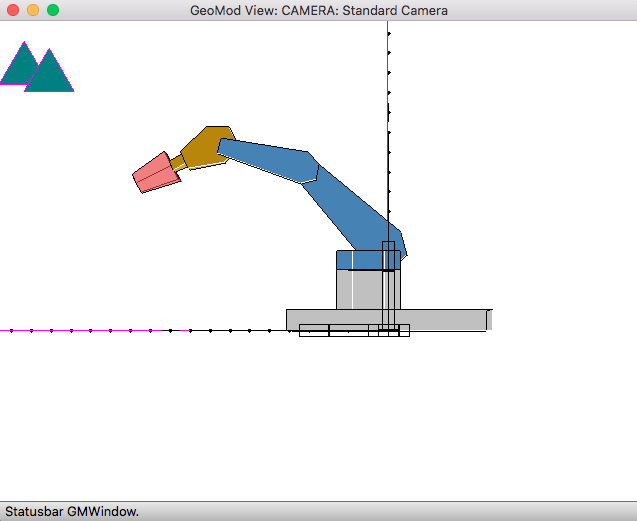
\includegraphics[height=8cm]{images/GeometricModel.png}
    \caption[Geometric model of a serial manipulator]{Geometric model of a serial manipulator}
    \label{fig:SerialManipulator}
\end{figure}


\section{Kinematics}
It was mentioned that from the work of Martin Lygre Fuglevik, the control system for desired position and orientation of objects along a network of paths was partially implemented. Most of the implementation worked as it should, but some occurrence regarding rotation in motion to a particular path did not work as prompted. Some small alteration had to be done in the model in order to continue the implementation of the control system. 

\begin{figure}[ht]
    \centering
    \includegraphics[height=8cm]{images/Diagram_Serial_Manipulator.png}
    \caption[Kinematic connection of  each part of the serial manipulator model]{Kinematic connection of  each part of the serial manipulator model}
    \label{fig:KinematicsSerialManipulator}
\end{figure}


The \Cref{fig:KinematicsSerialManipulator} illutrates how the forward and inverse kinematics works on the implemented model. This is done by having variables over the position, rotation and angle on each part of the model. The angle is determined by linking the parts from the base. By applying forward kinematics, the joints angle is independently controlled for each parts beginning from the position of the linked mechanism, the bracket, to end-effector, the gripper. The function \textit{dirKin()} is an already implemented function that calculate joint angels of all the joints, when one of the joints is moved. This makes a lot of unnecessary computation regarding to joints that are not affected of certain movement. This was disregarded as it did not prevent the objective of this project, but should be taken into account in future for optimization. Forward kinematics works well for a desired end position for the end-effector, but is rather impractical to control when following a path.

To work along network of path, a UAV is prompted to work in a specific area. This means the end-effector of a robot arm on the UAV follow a path as it doing its task. 




\chapter{Discussion}

\section{Further Work}



\chapter{Conclusion}

\section{test}




% Bibliography - edit references.bib and use the \cite command in text
\renewcommand{\bibname}{References}
\bibliographystyle{plain}
\bibliography{references}
%\addcontentsline{toc}{chapter}{\bibname}

\clearpage
\clearpage
\vspace*{\fill}
{\centering\huge\bfseries Appendix \par}
\vspace*{\fill}

\phantomsection
\addcontentsline{toc}{chapter}{Appendix}

\pagenumbering{arabic}% resets `page` counter to 1
\renewcommand*{\thepage}{A-\arabic{page}}

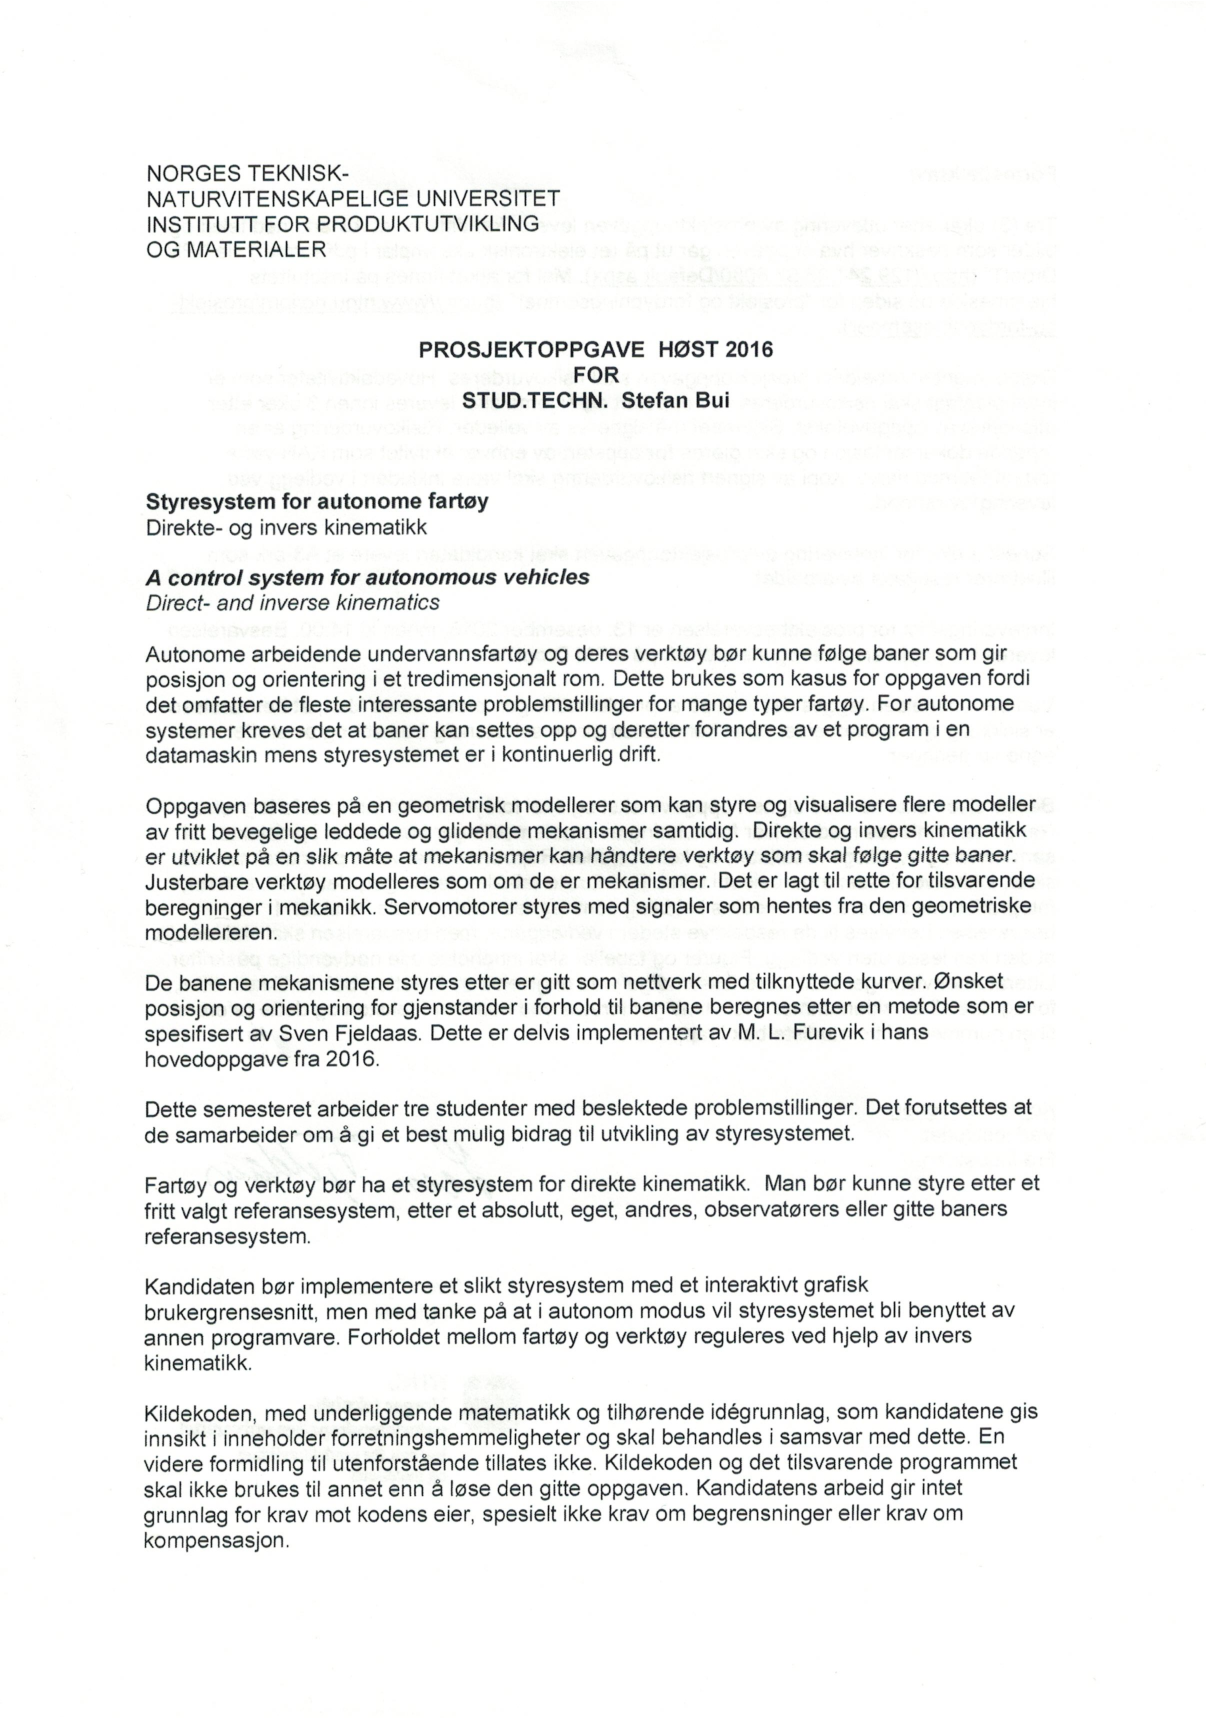
\includepdf[pages=-]{appendix/pdf/assignment.pdf}

%\addcontentsline{toc}{chapter}{B Project Assignment}
\includepdf[pages=2]{appendix/pdf/assignment.pdf}
%\addcontentsline{toc}{chapter}{C Risk Assessment}

\end{document}
